\documentclass[a4paper; 11pt]{article}
\usepackage[utf8]{inputenc}
\usepackage[english]{babel}
\usepackage{graphicx}
\usepackage{multicol}
\usepackage{amsmath}
\makeatletter
\setlength{\@fptop}{0pt}
\makeatother
\setlength{\columnsep}{1cm}
\bibliographystyle{unsrt}
\begin{document}

\title{Usability of Mobile Map Applications}

\author{Rachel Rivera\\
Professor: Dr. Dionisio\\
CMSI 370: Interaction Design\\
  Loyola Marymount University}

\date{September 25, 2014}

% Create title page with no page number

\renewcommand{\thefootnote}{\fnsymbol{footnote}}



%\singlespacing

\maketitle

\vspace{-.2in}
\begin{center}
\begin{abstract}
\noindent This investigation is motivated by the increasing significance of the usability of systems in today's competitive technology market. Usability testing and usability evaluations have become important tools in the assessment of user interfaces. This paper presents empirical mobile usability studies of two distinct map applications: Google Maps and Apple Maps. Participants of this investigation were asked to carry out three tasks with each mobile map application. The results of this examination include (a) the contextual factors studied; (b) quantitative data collected from each task; (c) a brief qualitative review of the applications from each participant; and (d) the core usability metrics measured. This paper not only presents the usability metrics collected by the study but also presents a heuristic evaluation of each map application.
\end{abstract}
\end{center}

\medskip
\medskip


\medskip
\noindent \textit{Group Members}: Katarina Klask, J.B. Morris, Alex Schneider, Khalid Seirafi, and Ronald Uy.

\thispagestyle{empty}

\clearpage

%\onehalfspacing
\setcounter{footnote}{0}
\renewcommand{\thefootnote}{\arabic{footnote}}
\setcounter{page}{1}

\section{Introduction}
When the Apple Maps mobile application was first released as part of iOS 6 in September 2012, it received a significant amount of negative feedback. Walt Mossberg of the \textit{Wall Street Journal} was one of many who thought that Apple Maps was the biggest drawback of the iPhone 5.\cite{Mossberg} At this time, the Google Maps mobile apps, on both iOS and Android, were used by roughly 81 million people.\cite{ComScore} However, Apple Maps grew, matured, and began gaining traction. By September 2013, Apple Maps gained 35 million regular users. The number of users of Google Maps dropped to around 58.7 million at this time.\cite{ComScore} Although the Apple Maps mobile app is newer than the Google Maps mobile app,\footnote{The initial release of Google Maps for Mobile was in September of 2008.} the two map applications are comparable with respect to features they provide as well as popularity nowadays.
\medskip
\par
Since both Google Maps apps and Apple Maps apps are widely known and used, it is important that the usability metrics of the two systems are examined. Thus, this study aims to empirically investigate the usability of each application. The current consensus within the field of interaction design is that usability depends on five distinct metrics: \textit{learnability}, \textit{efficiency}, \textit{errors}, \textit{memorability}, and \textit{satisfaction}.\cite{Nielsen} The three metrics that this particular study focuses on are efficiency, errors, and satisfaction.
\section{Contextual Factors}
Prior to having each test subject perform the tasks, a little contextual data about the users was first collected. Users were asked about their previous experience with Apple Maps, their previous experience with Google Maps, and their overall technological proficiency.
\vspace{-.2in}
\begin{figure}[ht]
\begin{center}
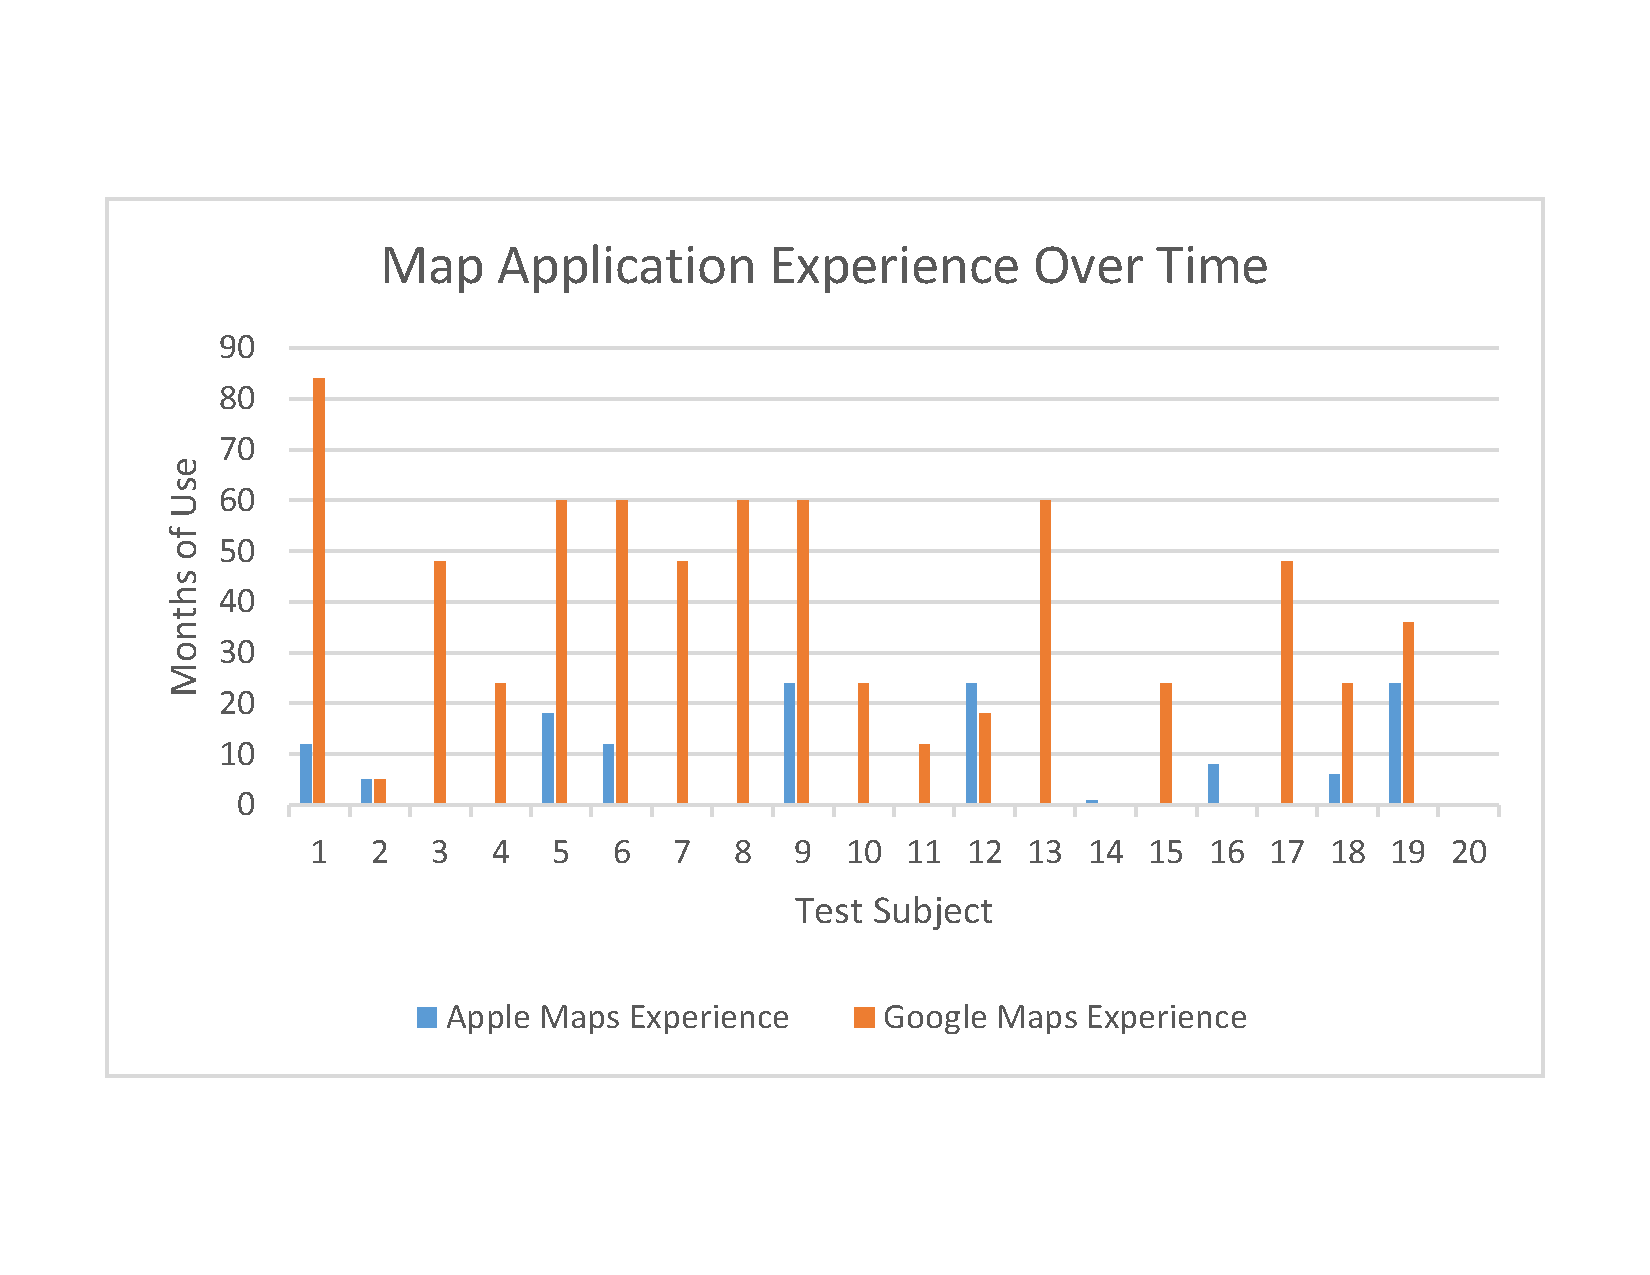
\includegraphics[keepaspectratio, width=.7\textwidth ]{user_context.pdf}
\end{center}
\end{figure}
\clearpage
\par
The fact that nearly every test subject had significantly more Google Maps experience than Apple Maps experience was a challenge in the conducting of this study.  Since this study aimed to test the usability metric of efficiency, and not that of learnability, we did not test subjects if they had no prior experience with the application. For future studies, however, it might be worthwhile to give inexperienced users a short tutorial so it is possible to test them thereafter.



\section{The Experiment} \label{sec:Experiment}
Each person who participated in this study had to carry out three concrete tasks with each of the map applications.
\begin{enumerate}
  \item Save a pin anywhere on the map and get driving directions to that pin.
  \item Find the location of the nearest Vons.
  \item Find the fastest route from the current location to LACMA.
\end{enumerate}
In order to keep the study as controlled as possible, all testing was done on iOS devices (no map applications of android devices were tested). As test subjects executed the tasks, information was collected pertaining to their efficiency, errors, and satisfaction.


\section{Usability Metrics}
\subsection{Efficiency}
\par
\textbf{First Task: }Drop a pin on the map and get driving directions to that pin.
\vspace{-.4in}
\begin{figure}[ht]
\begin{center}
\vspace{-.1in}
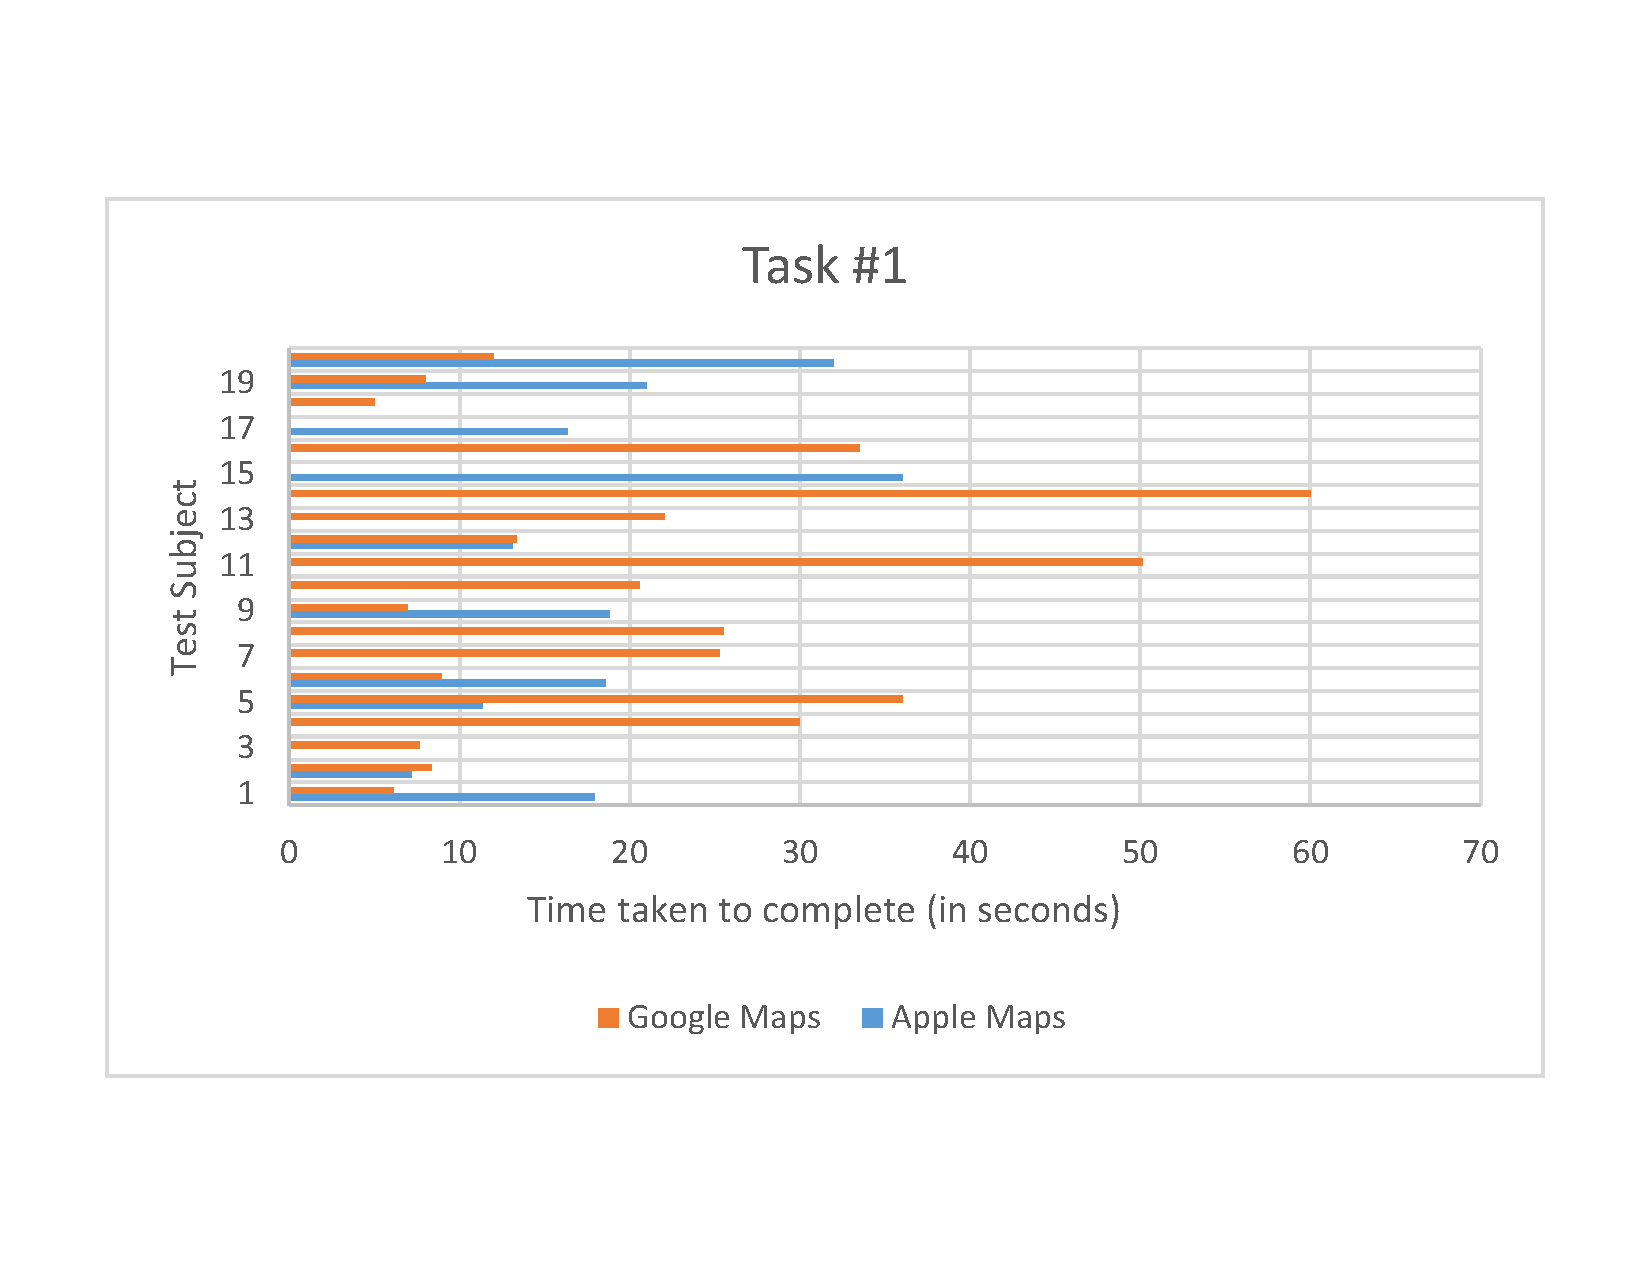
\includegraphics[keepaspectratio, width=.8\textwidth ]{task1.pdf}
\end{center}
\end{figure}
\begin{center}
\vspace{-.6in}
\par
Average time for task \#1 on Apple Maps app: approx. \textit{19 seconds}
\par
Average time for task \#1 on Google Maps app: approx. \textit{21 seconds}
\end{center}
\par
\noindent
This task's results suggest that users are more efficient using Apple Maps. \footnote{Though subjects using Apple Maps were more efficient \textit{on average}, it is important to note that there were a couple of anomalies within the set of Google Maps users.}
\medskip
\medskip
\par
\noindent
\textbf{Second Task: }Find the location of the nearest Vons.
\begin{figure}[ht]
\begin{center}
\vspace{-.5in}
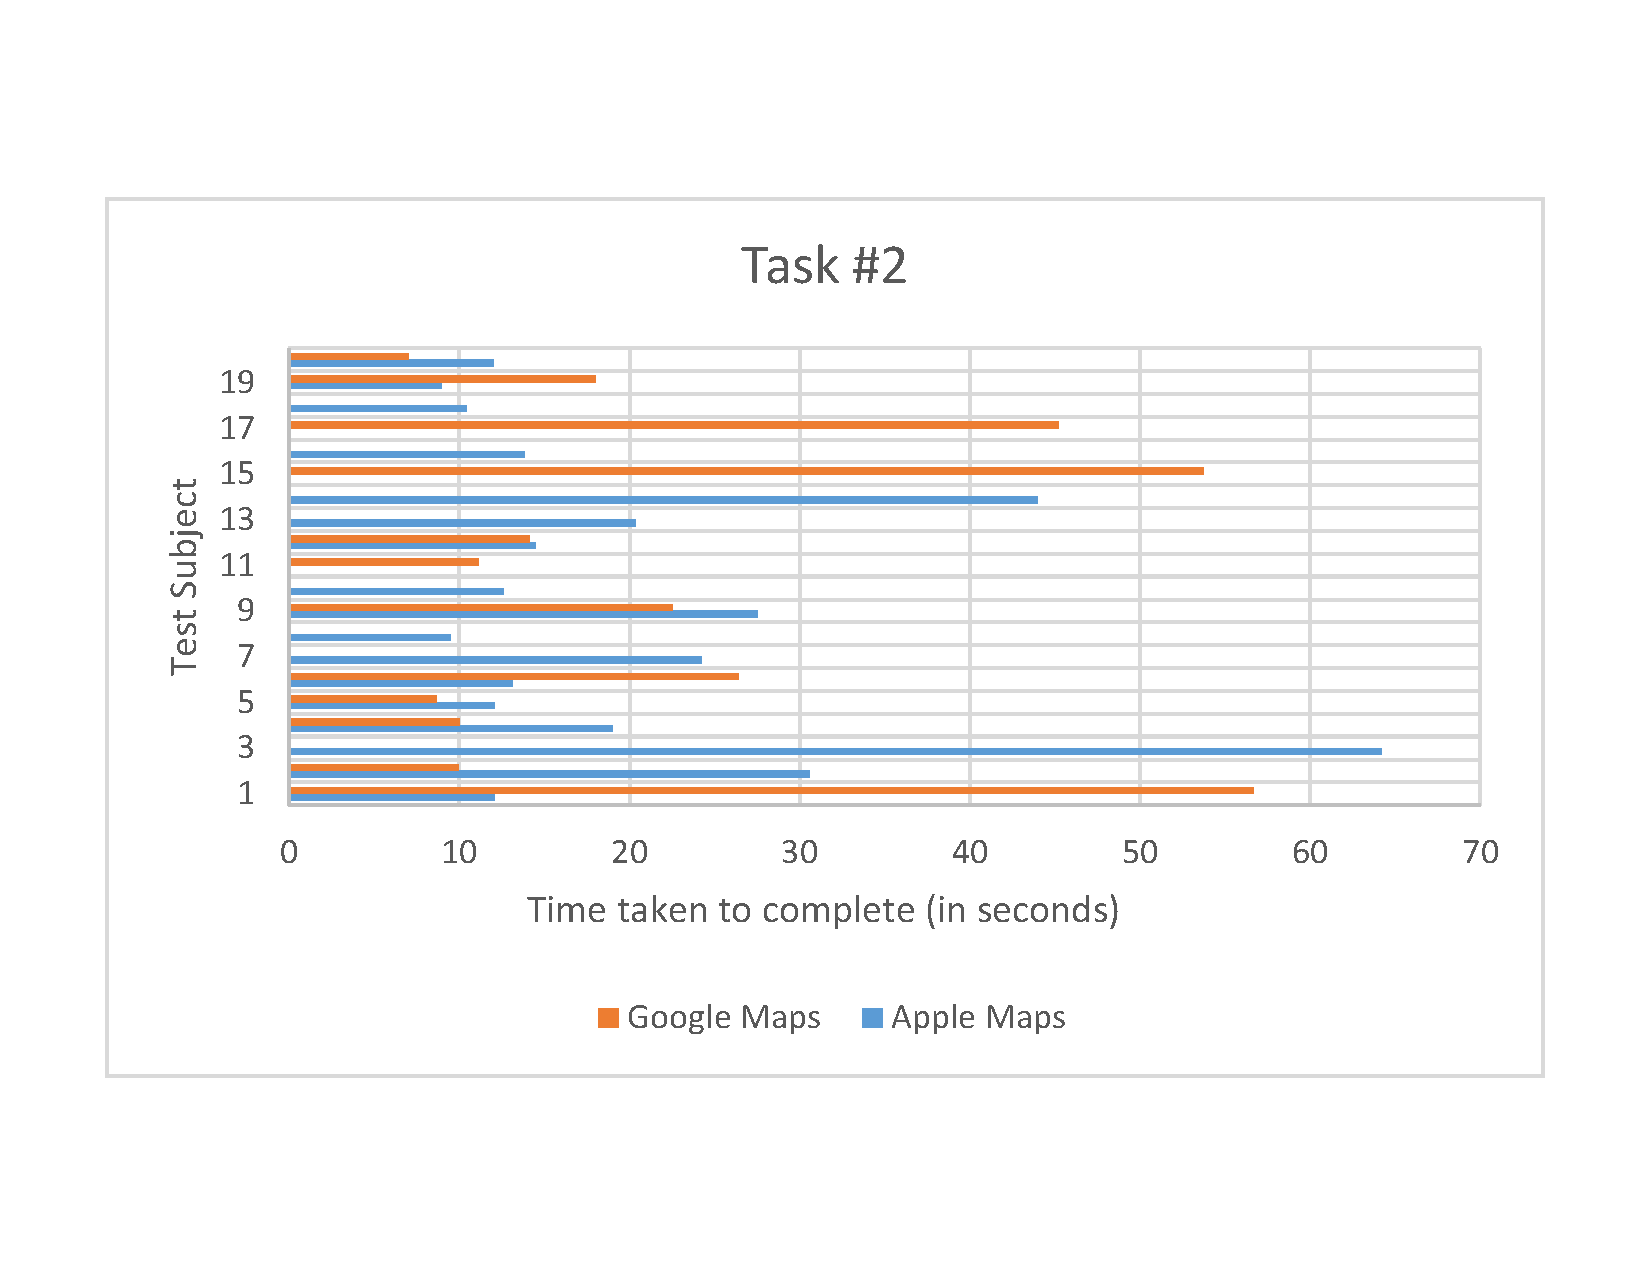
\includegraphics[keepaspectratio, width=.8\textwidth ]{task2.pdf}
\end{center}
\end{figure}
\begin{center}
\vspace{-.6in}
\par
Average time for task \#2 on Apple Maps app: approx. \textit{24 seconds}
\par
Average time for task \#2 on Google Maps app: approx. \textit{21 seconds}
\end{center}
\par
\noindent
This task's results suggest that users are more efficient using Google Maps. 
\medskip
\medskip
\par
\noindent
\textbf{Third Task: }Find the fastest route from the current location to LACMA.
\begin{figure}[ht]
\begin{center}
\vspace{-.4in}
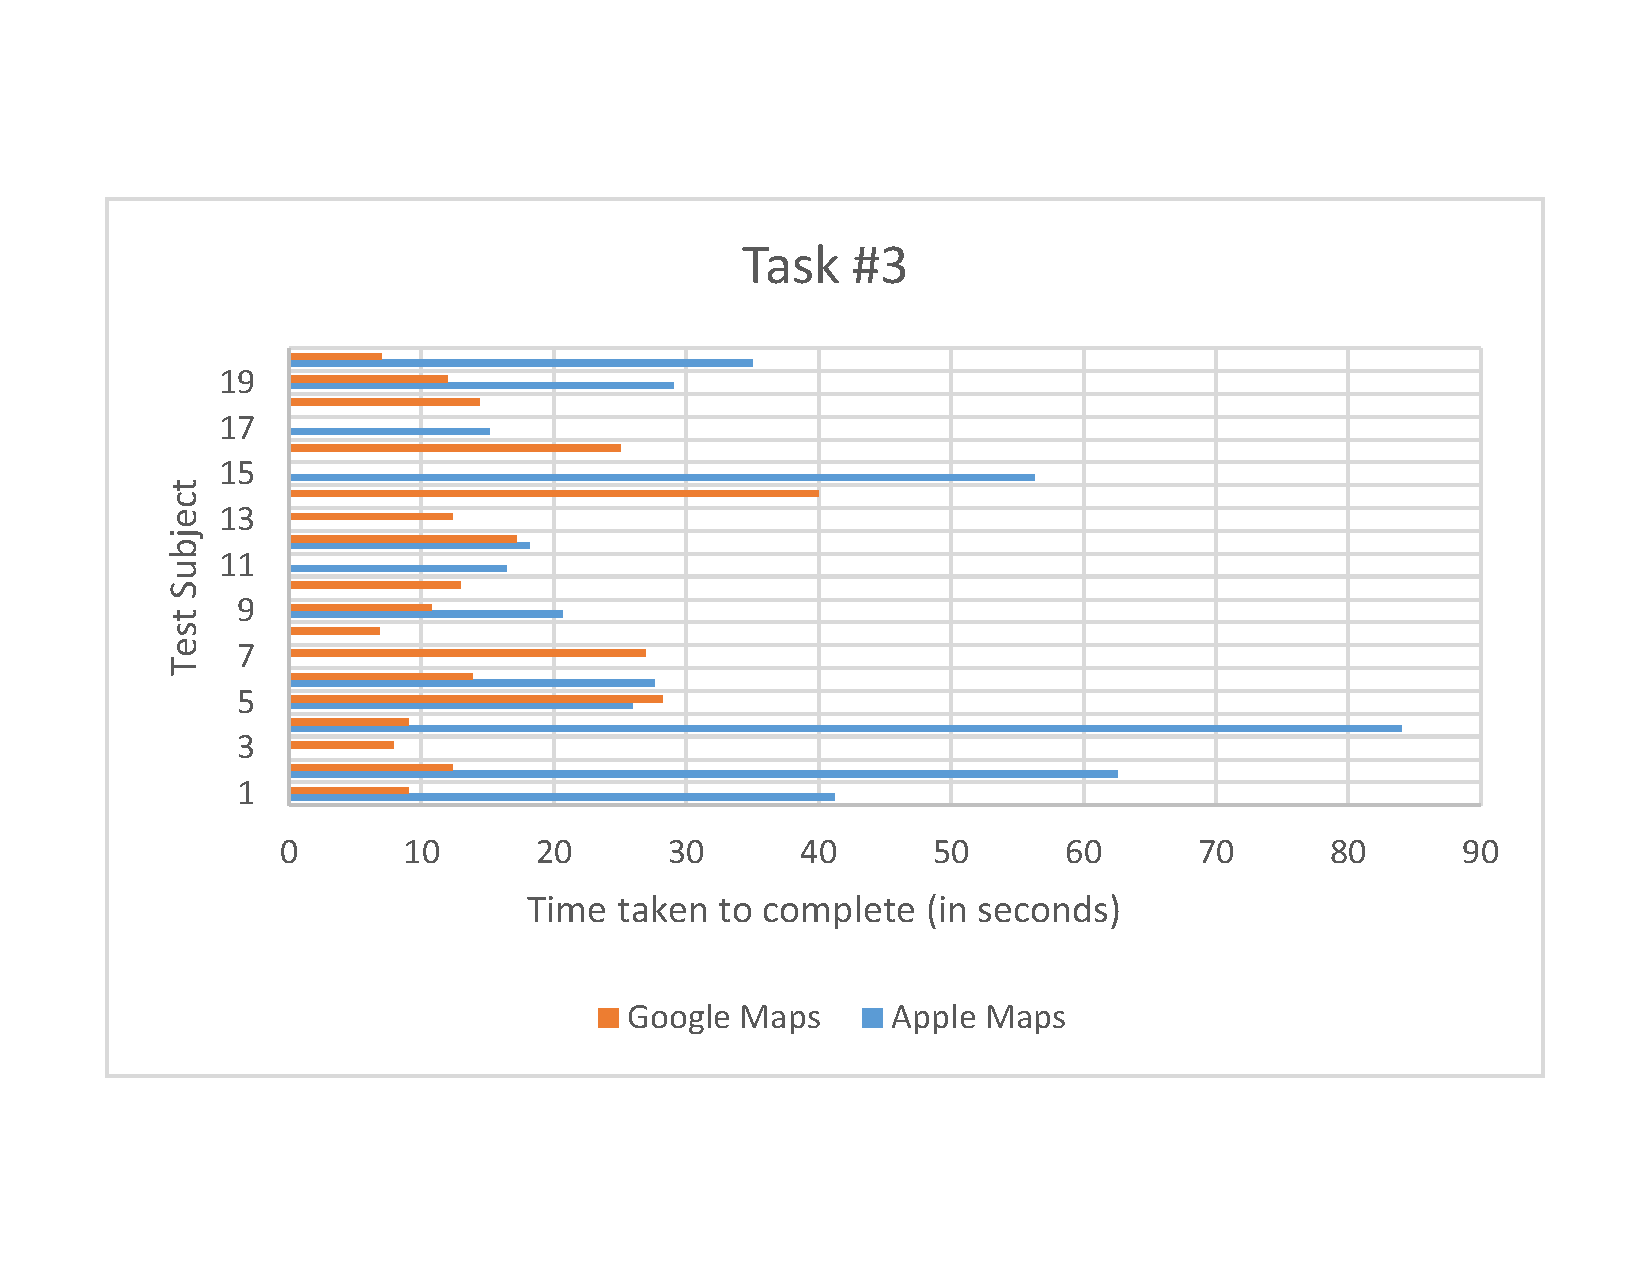
\includegraphics[keepaspectratio, width=.8\textwidth ]{task3.pdf}
\end{center}
\end{figure}
\begin{center}
\vspace{-.4in}
\par
Average time for task \#3 on Apple Maps app: approx. \textit{36 seconds}
\par
Average time for task \#3 on Google Maps app: approx. \textit{17 seconds}
\end{center}
\par
\noindent
This task's results suggest that users are more efficient using Google Maps. 

\subsection{Errors}
\par
The only errors collected by this study were incidents wherein the user did something whose result is not what he or she anticipated. The table on the following page shows you some examples of errors from this investigation.

\begin{table}[ht]
\centering
\begin{tabular}{l|c|c}
Task & Application & Specific Error\\\hline
Task1 & Apple Maps & hit \textit{Share} button; no response from tapping \\
Task1 & Google Maps & hit \textit{Near You} button to try to drop pin\\
Task2 & Apple Maps & tried to manually search for ``Nearest Vons"\\
Task2 & Google Maps & voice command instead of search\\
Task3 & Apple Maps & hit \textit{Current Location} for directions\\
Task3 & Google Maps & found side streets when expecting highway route
\end{tabular}
\end{table}
\par
The \textit{percentage} of subjects with errors is analyzed rather than solely the numbers of errors since more subjects tested the Google Maps app than Apple Maps app.
\begin{table}[ht]
\begin{tabular}{l c c c c}
& \multicolumn{4}{c}{}\\ % Amalgamating several columns into one cell is done using the \multicolumn command as seen on this line
& \textbf{Task1} & \textbf{Task2} & \textbf{Task3} \\
Percentage of Apple Users with Errors & 40\% & 50\%  & 20\% \\
Percentage of Google Users with Errors & 29.4\% & 17.6\%  & 11.7\% \\

\end{tabular}

\end{table}
\par
The results suggest that Google Maps is more usable with respect to errors.

\subsection{Satisfaction}
\begin{figure}[ht]
\begin{center}
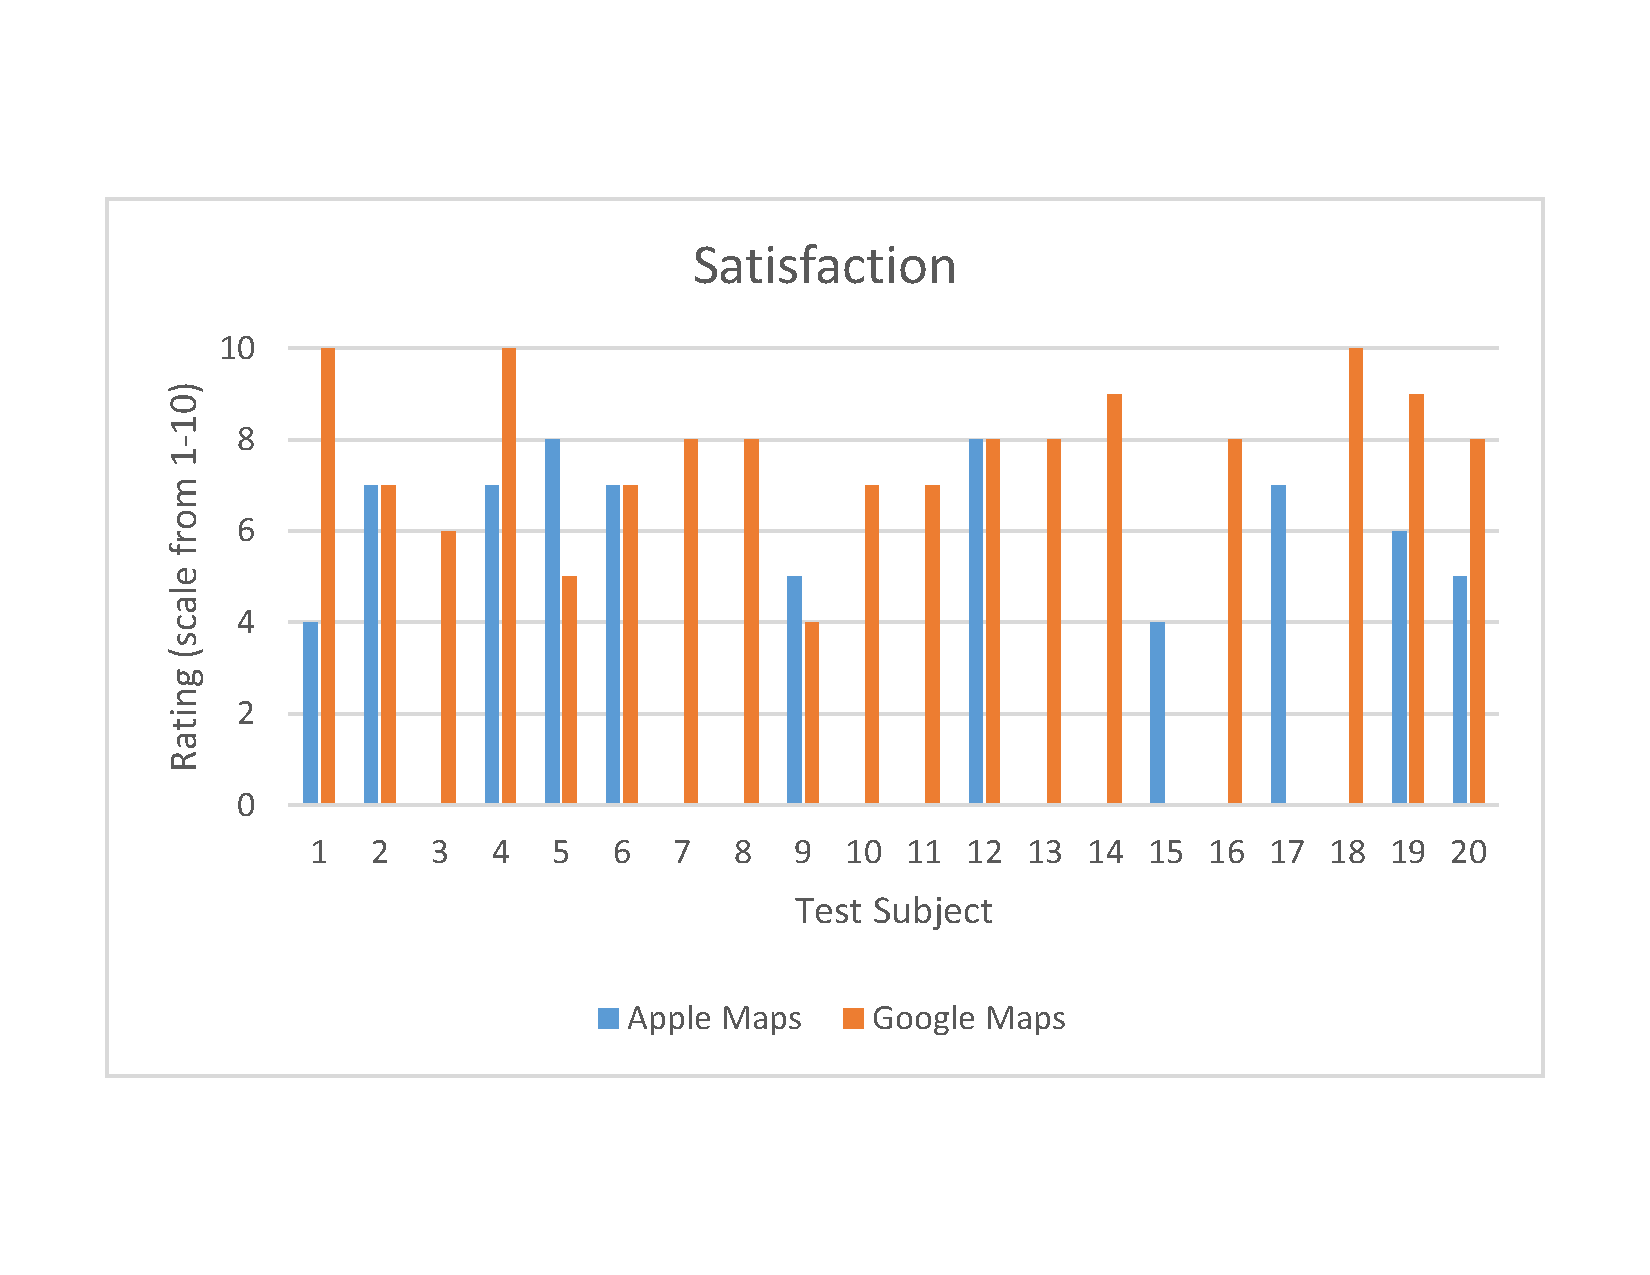
\includegraphics[keepaspectratio, width=.8\textwidth ]{satisfaction.pdf}
\end{center}
\end{figure}
\par
Satisfaction ratings were on a scale from 1 to 10.
\par
Average rating for Apple Maps: approx. \textbf{6.18}
\par
Average rating for Google Maps: approx. \textbf{7.72}

\begin{multicols}{2}
[
\section{Heuristic Evaluation}
All human things are subject to decay. And when fate summons, Monarchs must obey.
]
Hello, here is some text without a meaning.  This text should show what 
a printed text will look like at this place.
If you read this text, you will get no information.  Really?  Is there 
no information?  Is there
\end{multicols}
\clearpage
\begin{thebibliography}{100} % 100 is a random guess of the total number of 
%references
\bibitem{Nielsen} Nielsen, Jakob, \emph{Usability Engineering}, Boston: Academic, 1993.
\bibitem{Mossberg} Mossberg, Walt., ``The iPhone Takes to the Big Screen," \emph{The Wall Street Journal}, September 2012.
\bibitem{ComScore}``Analytics for a Digital World - ComScore, Inc." \emph{ComScore,Inc}, 2012.
\bibitem{HK} Kopka, H., Daly P.W., \emph{A Guide to LaTeX},
Addison-Wesley, Reading, MA, 1999.
\bibitem{Pan} Pan, D., ``A Tutorial on MPEG/Audio Compression," \emph{IEEE 
Multimedia}, Vol.2, pp.60-74, Summer 1998.
\end{thebibliography}
%%%%%%%%%%%%% end %%%%%%%%%%%%%%%%%%%%%%%%%%%%%%%



\end{document}